\subsection{Sequence Diagram}
\begin{figure}[H]

\fbox{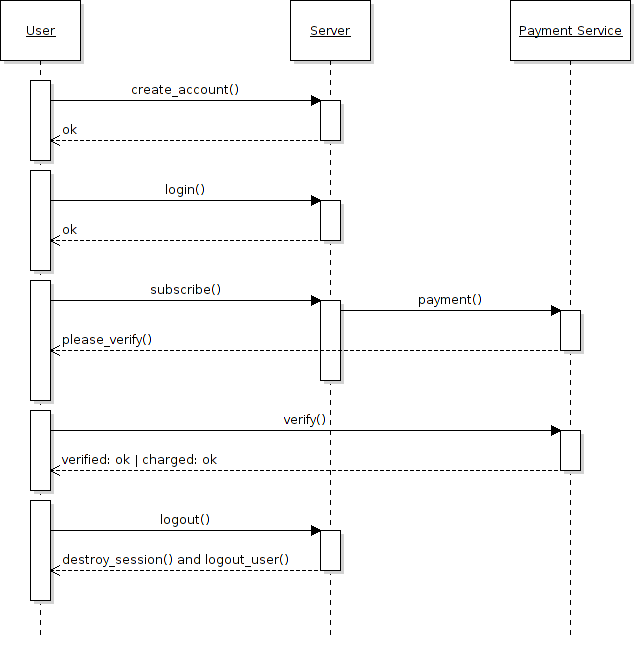
\includegraphics[scale=0.65]{graphics/sequence_diagram}}
\caption{Sequence Diagram (subscription and payment)}
\end{figure}

In order to add a subscription to an user account, the user obviously has to register an account and login to the member-only page.\\
Once this is done the user can request access to a feature which is "pay-to-use" by invoking the subscribe() method.\\
The server will then send a request to the payment service' servers (ie. VISA/Mastercard) and ask them to charge the user a specific amount of money.\\
\\
But before the user is charged, the user has to verify using for example OpenID.
Once this verification process has finalized, the user is charged and sent back to member-only page.\\
\\
The user can then start using the "pay-to-use" functionality or, as shown in the diagram, log out of the application.